% f2015hbl_q15_tangent.tex — 2015 年高考数学·湖北卷·理科 第 15 题（圆切线割线）
%
% 【来源】`.work/phase3-b21/source/2015湖北理.pdf`（SHA-256
%   66e6822009bdfd8f9a5a4adf4dd3f7564fc74d8fa09906c271dc6c6a5b31a66f），
%   第 1 页（合订本页 951）；内容对象 5/7/9/…/19。逐路径实测见
%   `.work/phase3-b21/figure-inventory.md`。
%
% 【坐标口径】源 PDF 用户空间（原点左下、y 向上）。本图本地坐标
%   (x, y) = (x_page − 903.944, y_page − 563.065)，1 单位 = 1 TeX pt。
%   路径坐标逐点照录内容流（含三次贝塞尔控制点）。
%
% 元素计数：4 条路径（圆、割线 P–B–C、弦 C–A、切线 P–A）＋4 个标签
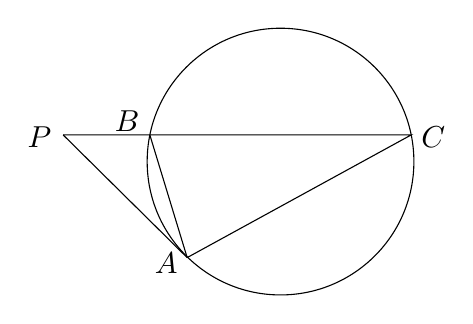
\begin{tikzpicture}[x=1pt, y=1pt,
    every node/.style={inner sep=0pt, font=\fontsize{10.5pt}{12.6pt}\selectfont}]
  \draw[line width=0.398pt] (126.7385,48.1890)   .. controls (126.7385,74.8040) and (105.1635,96.3780) .. (78.5495,96.3780)   .. controls (51.9345,96.3780) and (30.3595,74.8040) .. (30.3595,48.1890)   .. controls (30.3595,21.5740) and (51.9345,0.0000) .. (78.5495,0.0000)   .. controls (105.1635,0.0000) and (126.7385,21.5740) .. (126.7385,48.1890)   -- cycle;
  \draw[line width=0.398pt] (-0.0001,57.8267)   -- (125.7749,57.8267)   -- (44.8169,13.4927);
  \draw[line width=0.398pt] (31.3235,57.8267)   -- (44.8165,13.4927);
  \draw[line width=0.398pt] (-0.0001,57.8267)   -- (44.8169,13.4927);

  \node[anchor=center] at (-8.544,56.875) {$P$};  % 源中心 (895.40,619.94)
  \node[anchor=center] at (37.206,11.575) {$A$};  % 源中心 (941.15,574.64)
  \node[anchor=center] at (133.706,56.875) {$C$};  % 源中心 (1037.65,619.94)
  \node[anchor=center] at (23.106,62.675) {$B$};  % 源中心 (927.05,625.74)

\end{tikzpicture}
%
% 【自验结果】
%   探针：latexmk -pdfxe（待跑）。
